\documentclass[journal,12pt,twocolumn]{IEEEtran}
%
\usepackage{setspace}
\usepackage{gensymb}
\usepackage{tkz-euclide} 
\usepackage{textcomp}
\usepackage{standalone}
\usetikzlibrary{calc}
\usepackage{float}
%\doublespacing
\singlespacing

%\usepackage{graphicx}
%\usepackage{amssymb}
%\usepackage{relsize}
\usepackage[cmex10]{amsmath}
%\usepackage{amsthm}
%\interdisplaylinepenalty=2500
%\savesymbol{iint}
%\usepackage{txfonts}
%\restoresymbol{TXF}{iint}
%\usepackage{wasysym}
\usepackage{amsthm}
%\usepackage{iithtlc}
\usepackage{mathrsfs}
\usepackage{txfonts}
\usepackage{stfloats}
\usepackage{bm}
\usepackage{cite}
\usepackage{cases}
\usepackage{subfig}
%\usepackage{xtab}
\usepackage{longtable}
\usepackage{multirow}
%\usepackage{algorithm}
%\usepackage{algpseudocode}
\usepackage{enumitem}
\usepackage{mathtools}
\usepackage{steinmetz}
\usepackage{tikz}
\usepackage{circuitikz}
\usepackage{verbatim}
\usepackage{tfrupee}
\usepackage[breaklinks=true]{hyperref}
%\usepackage{stmaryrd}
\usepackage{tkz-euclide} % loads  TikZ and tkz-base
%\usetkzobj{all}
\usetikzlibrary{calc,math}
\usepackage{listings}
    \usepackage{color}                                            %%
    \usepackage{array}                                            %%
    \usepackage{longtable}                                        %%
    \usepackage{calc}                                             %%
    \usepackage{multirow}                                         %%
    \usepackage{hhline}                                           %%
    \usepackage{ifthen}                                           %%
  %optionally (for landscape tables embedded in another document): %%
    \usepackage{lscape}     
\usepackage{multicol}
\usepackage{chngcntr}
\usepackage{romannum}
%\usepackage{enumerate}
%\usepackage{wasysym}
%\newcounter{MYtempeqncnt}
\DeclareMathOperator*{\Res}{Res}
%\renewcommand{\baselinestretch}{2}
\renewcommand\thesection{\arabic{section}}
\renewcommand\thesubsection{\thesection.\arabic{subsection}}
\renewcommand\thesubsubsection{\thesubsection.\arabic{subsubsection}}

\renewcommand\thesectiondis{\arabic{section}}
\renewcommand\thesubsectiondis{\thesectiondis.\arabic{subsection}}
\renewcommand\thesubsubsectiondis{\thesubsectiondis.\arabic{subsubsection}}

% correct bad hyphenation here
\hyphenation{op-tical net-works semi-conduc-tor}
\def\inputGnumericTable{}                                 %%

\lstset{
%language=C,
frame=single, 
breaklines=true,
columns=fullflexible
}
%\lstset{
%language=tex,
%frame=single, 
%breaklines=true
%}

\begin{document}
%


\newtheorem{theorem}{Theorem}[section]
\newtheorem{problem}{Problem}
\newtheorem{proposition}{Proposition}[section]
\newtheorem{lemma}{Lemma}[section]
\newtheorem{corollary}[theorem]{Corollary}
\newtheorem{example}{Example}[section]
\newtheorem{definition}[problem]{Definition}
%\newtheorem{thm}{Theorem}[section] 
%\newtheorem{defn}[thm]{Definition}
%\newtheorem{algorithm}{Algorithm}[section]
%\newtheorem{cor}{Corollary}
\newcommand{\BEQA}{\begin{eqnarray}}
\newcommand{\EEQA}{\end{eqnarray}}
\newcommand{\define}{\stackrel{\triangle}{=}}
\bibliographystyle{IEEEtran}
%\bibliographystyle{ieeetr}
\providecommand{\mbf}{\mathbf}
\providecommand{\pr}[1]{\ensuremath{\Pr\left(#1\right)}}
\providecommand{\qfunc}[1]{\ensuremath{Q\left(#1\right)}}
\providecommand{\sbrak}[1]{\ensuremath{{}\left[#1\right]}}
\providecommand{\lsbrak}[1]{\ensuremath{{}\left[#1\right.}}
\providecommand{\rsbrak}[1]{\ensuremath{{}\left.#1\right]}}
\providecommand{\brak}[1]{\ensuremath{\left(#1\right)}}
\providecommand{\lbrak}[1]{\ensuremath{\left(#1\right.}}
\providecommand{\rbrak}[1]{\ensuremath{\left.#1\right)}}
\providecommand{\cbrak}[1]{\ensuremath{\left\{#1\right\}}}
\providecommand{\lcbrak}[1]{\ensuremath{\left\{#1\right.}}
\providecommand{\rcbrak}[1]{\ensuremath{\left.#1\right\}}}
\theoremstyle{remark}
\newtheorem{rem}{Remark}
\newcommand{\sgn}{\mathop{\mathrm{sgn}}}
\providecommand{\abs}[1]{\left\vert#1\right\vert}
\providecommand{\res}[1]{\Res\displaylimits_{#1}} 
\providecommand{\norm}[1]{\left\lVert#1\right\rVert}
%\providecommand{\norm}[1]{\lVert#1\rVert}
\providecommand{\mtx}[1]{\mathbf{#1}}
\providecommand{\mean}[1]{E\left[ #1 \right]}
\providecommand{\fourier}{\overset{\mathcal{F}}{ \rightleftharpoons}}
%\providecommand{\hilbert}{\overset{\mathcal{H}}{ \rightleftharpoons}}
\providecommand{\system}{\overset{\mathcal{H}}{ \longleftrightarrow}}
	%\newcommand{\solution}[2]{\textbf{Solution:}{#1}}
\newcommand{\solution}{\noindent \textbf{Solution: }}
\newcommand{\cosec}{\,\text{cosec}\,}
\providecommand{\dec}[2]{\ensuremath{\overset{#1}{\underset{#2}{\gtrless}}}}
\newcommand{\myvec}[1]{\ensuremath{\begin{pmatrix}#1\end{pmatrix}}}
\newcommand{\mydet}[1]{\ensuremath{\begin{vmatrix}#1\end{vmatrix}}}
%\numberwithin{equation}{section}
\numberwithin{equation}{subsection}
%\numberwithin{problem}{section}
%\numberwithin{definition}{section}
\makeatletter
\@addtoreset{figure}{problem}
\makeatother
\let\StandardTheFigure\thefigure
\let\vec\mathbf
%\renewcommand{\thefigure}{\theproblem.\arabic{figure}}
\renewcommand{\thefigure}{\theproblem}
%\setlist[enumerate,1]{before=\renewcommand\theequation{\theenumi.\arabic{equation}}
%\counterwithin{equation}{enumi}
%\renewcommand{\theequation}{\arabic{subsection}.\arabic{equation}}
\def\putbox#1#2#3{\makebox[0in][l]{\makebox[#1][l]{}\raisebox{\baselineskip}[0in][0in]{\raisebox{#2}[0in][0in]{#3}}}}
     \def\rightbox#1{\makebox[0in][r]{#1}}
     \def\centbox#1{\makebox[0in]{#1}}
     \def\topbox#1{\raisebox{-\baselineskip}[0in][0in]{#1}}
     \def\midbox#1{\raisebox{-0.5\baselineskip}[0in][0in]{#1}}
\vspace{3cm}
\title{Assignment 5}
\author{Vinay kumar}
\maketitle
\newpage
Download all python codes
and latex-tikz codes from 
%
\begin{lstlisting}
https://github.com/jvinaykumar12/EE5609/tree/master/Assignment5
\end{lstlisting}
%
\section{Problem}
For what value of k does the equation 
\begin{align}
\vec{x}^T\myvec{12 & \frac{7}{2} \\ \frac{7}{2} & k}\vec{x} + \myvec{13 & -1}\vec{x} + 3 = 0 
\label{eq:a0}
\end{align}
represents a pair of straight lines and find the angle between the lines.
\section{Explanation}

Given equation is in the form 
\begin{align}
\vec{x}^T\vec{V}\vec{x} + 2\vec{u}^T + f = 0
\label{eq:a1}
\end{align}

Therefore by comparing, we get
\begin{align}
&\vec{V} = \myvec{12 & \frac{7}{2} \\ \frac{7}{2} & k} \label{eq:a2}\\
&\vec{u} = \myvec{\frac{13}{2} \\ \frac{-1}{2}}  \\
&f = 3 
\end{align}

Equation \eqref{eq:a0} represents pair of two straight lines, if 

\begin{align}
&\mydet{\vec{V} & \vec{u} \\ \vec{u}^T & f} = 0 \\
&\mydet{12 & \frac{7}{2} & \frac{13}{2} \\ \frac{7}{2} & k & \frac{-1}{2} \\ \frac{13}{2} & \frac{-1}{2} & 3} = 0
\end{align}

By expanding the determinent, we get 

\begin{align}
k = -10 
\end{align}

Therefore, when the value of k is -10, the equation represents pair of straight lines and the equations of the two lines can be written as 

\begin{align}
&\vec{n_1}^T\vec{x} - c1 = 0 
&\vec{n_2}^T\vec{x} - c2 = 0
\label{eq:a3}
\end{align}

The above pair of lines can be represnted as 
\begin{multline}
(\vec{n_1}^T\vec{x} - c1)(\vec{n_2}^T\vec{x} - c2) = \vec{x}^T\vec{V}\vec{x} + 2\vec{u}^T + f  \\
ax^2+2bxy+cy^2+2dx+2ey+f=0
\end{multline}

By observation, we can written 
\begin{align}
&\vec{V} = \myvec{a & b \\ b & c}
&\vec{n_1}c_2 + \vec{n_2}c_1 =  -2\vec{u}   \\ 
&\vec{n_1}*\vec{n_2}  = \myvec{a \\ 2b \\ c} 
\end{align}

The slopes of the two lines are given by the roots of the polynomial 
\begin{align}
cm^2+2bm+a = 0 
\end{align}

The roots of the above equation is given by
\begin{align}
m = \frac{-b\pm{\sqrt{-\mydet{\vec{V}}}}}{c}
\label{eq:a4}
\end{align}

By replacing the values in \eqref{eq:a4} we get,
\begin{align}
\vec{m_1} = \myvec{5 \\ -4}
\vec{m_2} = \myvec{2 \\ 3} \\
\implies\vec{n_1} = \myvec{4 \\ 5} 
\vec{n_2} = \myvec{3 \\ -2}
\label{eq:a5}
\end{align}

Verification using Toeplitz matrix. From \eqref{eq:a5} 
\begin{align}
\vec{n_1} = \myvec{4 & 0 \\ 5 & 4 \\ 0 & 5 } 
\vec{n_2} = \myvec{3 \\ -2}    \\
\vec{n_1}*\vec{n_2} = \myvec{4 & 0 \\ 5 & 4 \\ 0 & 5 }\myvec{3 \\ -2} \\ 
= \myvec{12 \\ 7 \\ -10} = \myvec{a \\ 2b \\ c}
\end{align}

we know that 
\begin{align}
&\myvec{\vec{n_1} & \vec{n_2}}\myvec{c_2 \\ c_1} = -2\vec{u} \\
\end{align}

Solving the above equation using augmented matrix
\begin{align}
\myvec{4 & 3 & -13 \\ 5 & -2 & 1}
\xleftrightarrow[]{R_2 \leftarrow 4R_2-5R_1}
\myvec{4 & 3 & -13 \\ 0 & -23 & 69}\\
\xleftrightarrow[]{R_2 \leftarrow -\frac{R_2}{23}}
\myvec{4 & 3 & -13 \\ 0 & 1 & -3}
\xleftrightarrow[]{R_1 \leftarrow R_1-3R_2}
\myvec{4 & 0 & -4 \\ 0 & 1 & -3}\\
\xleftrightarrow[]{R_1 \leftarrow \frac{R_1}{4}}
\myvec{1 & 0 & -1 \\ 0 & 1 & -3} \\
\implies  c_2 = -1  c_1 = -3
\end{align}

Therefore the equation of the two straight lines are
\begin{align}
\myvec{4 & 5}\vec{x} = -3 \\
\myvec{3 &-2}\vec{x} = -1
\end{align}

The angle between the lines can be obtained by 
\begin{align}
&\cos \theta  = \frac{\vec{n_1}^T\vec{n_2}}{\norm{\vec{n_1}}\norm{\vec{n_2}}} \\
&\cos \theta  = \frac{2}{\sqrt{533}} \\
&\theta = cos^{-1}\brak{\frac{2}{\sqrt{533}}}
\end{align}

\begin{figure}
\centering
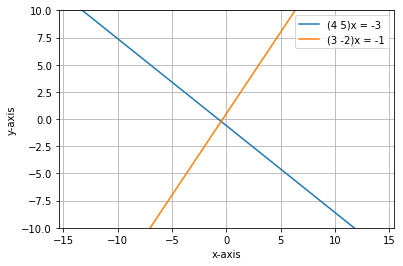
\includegraphics[width=\columnwidth]{Assignment5.png}
\caption{Plot showing the two lines }
\label{Fig 0}
\end{figure}

\end{document}
